\documentclass[10pt]{beamer}

% ------------------------------------------------------------------------
% Carga de tu preámbulo personalizado (preamble.tex).
% Asegúrate de tenerlo en la misma carpeta para que \input funcione.
% ------------------------------------------------------------------------
\usetheme[progressbar=frametitle]{metropolis}
\usepackage{appendixnumberbeamer}
\usepackage{fancyvrb}
\usepackage{booktabs}
\usepackage[scale=2]{ccicons}
\usepackage{pgfplots}
\usepgfplotslibrary{dateplot}
\usepackage{type1cm}
\usepackage{lettrine}
\usepackage{ragged2e}
\usepackage{xspace}
\newcommand{\themename}{\textbf{\textsc{metropolis}}\xspace}
\usepackage{graphicx} % Allows including images
\usepackage{booktabs} % Allows the use of \toprule, \midrule and \bottomrule in tables
\usepackage[utf8]{inputenc} %solucion del problema de los acentos.
\usepackage{xcolor}
\definecolor{LightGray}{gray}{0.9}

\usepackage{minted}
\usemintedstyle{tango}
\newcommand{\mypyfile}[1]{\inputminted[linenos=true, fontsize=\footnotesize, frame=lines, framesep=5\fboxrule,framerule=1pt]{python}{#1}}

\setminted[python]{breaklines,frame=lines,framesep=2mm,baselinestretch=1.2,bgcolor=LightGray,linenos, fontsize=\footnotesize} % obeytabs=true, tabsize=2, showtabs=true}

%%%%%%%%%%%%%%%%%%%%%%%%%%%%%%%%%%%%%%%%%%%%%%%%%%%%%%%%%%%%%%%%%%%%%%%%%%%%%%%%%%%%%%
\setbeamercolor{progress bar}{fg=blue!50!black,bg=white!50!black}
\setbeamercolor{title separator}{fg=red!50!black,bg=white!50!black}
\setbeamercolor{frametitle}{fg=white!80!black,bg=red!50!black}
\title[PCFI161]{Programaci\'on para F\'isica y Astronom\'ia}
\subtitle{Departamento de Física.}

\newcommand{\myfront}{
\author[PCFI161]{Corodinadora: C Loyola \\ Profesoras/es C Loyola / C Femenías / Y Navarrete / C Ruiz}
\institute[UNAB]{Universidad Andrés Bello}
\date{Primer Semestre 2025}
}

\titlegraphic{%
  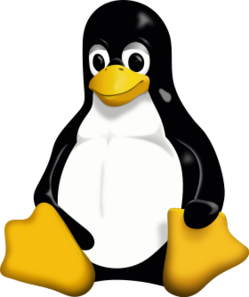
\includegraphics[width=.08\textwidth]{logo-tux.png}\hfill
  
\includegraphics[width=.3\textwidth]{logo-unab.png}\hfill
  
\includegraphics[width=.08\textwidth]{logo-python.png}
}

\makeatletter
\setbeamertemplate{title page}{
  \begin{minipage}[b][\paperheight]{\textwidth}
    \vfill%
    \ifx\inserttitle\@empty\else\usebeamertemplate*{title}\fi
    \ifx\insertsubtitle\@empty\else\usebeamertemplate*{subtitle}\fi
    \usebeamertemplate*{title separator}
    \ifx\beamer@shortauthor\@empty\else\usebeamertemplate*{author}\fi
    \ifx\insertdate\@empty\else\usebeamertemplate*{date}\fi
    \ifx\insertinstitute\@empty\else\usebeamertemplate*{institute}\fi
    \vfill
    \ifx\inserttitlegraphic\@empty\else\inserttitlegraphic\fi
    \vspace*{1cm}
  \end{minipage}
}
\makeatother


\makeatletter
\setlength{\metropolis@titleseparator@linewidth}{2pt}
\setlength{\metropolis@progressonsectionpage@linewidth}{2pt}
\setlength{\metropolis@progressinheadfoot@linewidth}{2pt}
\makeatother


\begin{document}

% ------------------------------------------------------------------------
% Portada de la Presentación
% ------------------------------------------------------------------------
\myfront{}

% ------------------------------------------------------------------------
% Slide 1: Título de la Sesión
% ------------------------------------------------------------------------
\begin{frame}
  \titlepage
  % Ejemplo:
  % \title{Semana 6 - Sesión 2 (Sesión 12): Operaciones Avanzadas con NumPy y Primeros Gráficos}
\end{frame}

% ------------------------------------------------------------------------
% Slide 2: Índice / Tabla de Contenidos
% ------------------------------------------------------------------------
\begin{frame}
  \frametitle{Resumen - Semana 6, Sesión 2 (Sesión 12)}
  \tableofcontents
\end{frame}

% ------------------------------------------------------------------------
% Configuración de bloques
% ------------------------------------------------------------------------
\metroset{block=fill}

% ----------------------------------------------------------------------------------------
% SECCIÓN 1: Repaso Breve de la Sesión Anterior
% ----------------------------------------------------------------------------------------
\section{Introducción y Repaso}

% ------------------------------------------------------------------------
% Slide 3: Repaso de la Sesión 11
% ------------------------------------------------------------------------
\begin{frame}{Repaso de la Sesión 11}
  \begin{itemize}
    \item Vimos la introducción a \textbf{NumPy} y creamos arreglos básicos.
    \item Exploramos:
      \begin{itemize}
        \item \texttt{np.array}, \texttt{np.zeros}, \texttt{np.arange}.
        \item Slicing, indexación y operaciones vectorizadas.
        \item Broadcasting con ejemplos simples.
      \end{itemize}
    \item Resolvimos ejercicios como la aproximación a \(\pi\) con la serie de Leibniz.
    \item \textbf{Objetivo de hoy}: Ampliar funciones avanzadas de NumPy, manipulación más compleja y daremos un primer vistazo a \textbf{Matplotlib} para gráficas.
  \end{itemize}
\end{frame}

% ------------------------------------------------------------------------
% Slide 4: Objetivos de la Sesión 12
% ------------------------------------------------------------------------
\begin{frame}{Objetivos de la Sesión 12}
  \begin{itemize}
    \item \textbf{Profundizar} en la manipulación de arrays: \texttt{reshape}, \texttt{transpose}, \texttt{concatenate}.
    \item \textbf{Explorar} funciones adicionales de \texttt{np.random} y \texttt{np.linalg}.
    \item \textbf{Iniciar} la transición a \textbf{visualizaciones} básicas con \textbf{Matplotlib}.
    \item \textbf{Aplicar} estos conceptos en ejercicios de simulación y análisis de datos sencillos.
  \end{itemize}
\end{frame}

% ----------------------------------------------------------------------------------------
% SECCIÓN 2: Manipulación Avanzada de Arrays
% ----------------------------------------------------------------------------------------
\section{Manipulación Avanzada de Arrays}

% ------------------------------------------------------------------------
% Slide 5: Reshaping
% ------------------------------------------------------------------------
\begin{frame}[fragile]{\texttt{reshape} para Cambiar Forma}
\begin{minted}{python}
import numpy as np

arr = np.arange(12)  # [0,1,2,...,11]
print("Arr 1D:", arr)

mat = arr.reshape((3,4))  # 3 filas, 4 columnas
print("Matriz 3x4:\n", mat)
\end{minted}
\begin{itemize}
  \item \textbf{reshape} no crea una copia, sino una vista (si posible).
  \item Dimensiones deben \textbf{coincidir} en la cantidad total de elementos.
\end{itemize}
\end{frame}

% ------------------------------------------------------------------------
% Slide 6: Transposición
% ------------------------------------------------------------------------
\begin{frame}[fragile]{\texttt{transpose} o \texttt{.T} para Matrices}
\begin{minted}{python}
mat = np.array([[1,2,3],
                [4,5,6]])
print("Original:\n", mat)

transpuesta = mat.T
print("Transpuesta:\n", transpuesta)

# También se puede usar:
# np.transpose(mat)
\end{minted}
\begin{itemize}
  \item Cambia ejes (filas pasan a ser columnas y viceversa).
\end{itemize}
\end{frame}

% ------------------------------------------------------------------------
% Slide 7: Concatenación de Arrays
% ------------------------------------------------------------------------
\begin{frame}[fragile]{\texttt{np.concatenate}, \texttt{np.vstack}, \texttt{np.hstack}}
\begin{minted}{python}
a = np.array([1,2,3])
b = np.array([4,5,6])

c = np.concatenate((a,b))
print("Concatenate 1D:", c)  # [1 2 3 4 5 6]

mat1 = np.array([[1,2],[3,4]])
mat2 = np.array([[5,6],[7,8]])

res_h = np.hstack((mat1, mat2))
# Horizontal: columnas se suman
print("Horizontal:\n", res_h)
# [[1 2 5 6]
#  [3 4 7 8]]

res_v = np.vstack((mat1, mat2))
# Vertical: filas se suman
print("Vertical:\n", res_v)
# [[1 2]
#  [3 4]
#  [5 6]
#  [7 8]]
\end{minted}
\end{frame}

% ----------------------------------------------------------------------------------------
% SECCIÓN 3: Funciones NumPy Random y Linalg
% ----------------------------------------------------------------------------------------
\section{Funciones Random y Linalg}

% ------------------------------------------------------------------------
% Slide 8: \texttt{np.random}
% ------------------------------------------------------------------------
\begin{frame}[fragile]{\texttt{np.random} para Valores Aleatorios}
\begin{minted}{python}
# Generar arreglo 1D de floats uniformes en [0,1)
rand_floats = np.random.rand(5)
print("Floats aleatorios:", rand_floats)

# Matriz 2x3 de flotantes uniformes
mat_uniform = np.random.rand(2,3)

# Enteros aleatorios en [low, high)
rand_ints = np.random.randint(low=1, high=10, size=5)
print("Enteros aleatorios [1..9]:", rand_ints)

# Fijar semilla para reproducibilidad
np.random.seed(42)
\end{minted}
\begin{itemize}
  \item \texttt{np.random.randn} para distribución normal estándar.
  \item \textbf{seed} para obtener siempre la misma secuencia.
\end{itemize}
\end{frame}

% ------------------------------------------------------------------------
% Slide 9: \texttt{np.linalg}
% ------------------------------------------------------------------------
\begin{frame}[fragile]{\texttt{np.linalg} para Álgebra Lineal}
\begin{minted}{python}
import numpy as np

A = np.array([[1,2],
              [3,4]])
# Determinante
detA = np.linalg.det(A)

# Inversa
invA = np.linalg.inv(A)

# Autovalores y autovectores
valores, vectores = np.linalg.eig(A)

print("Det(A) =", detA)
print("Inv(A) =\n", invA)
print("Eigenvalues =", valores)
print("Eigenvectors =\n", vectores)
\end{minted}
\begin{itemize}
  \item Módulo \texttt{linalg} (linear algebra) provee funcionalidad típica: inversas, resoluciones de sistemas, SVD, etc.
\end{itemize}
\end{frame}

% ----------------------------------------------------------------------------------------
% SECCIÓN 4: Primeros Pasos con Matplotlib
% ----------------------------------------------------------------------------------------
\section{Primeros Pasos con Matplotlib}

% ------------------------------------------------------------------------
% Slide 10: ¿Por qué Matplotlib?
% ------------------------------------------------------------------------
\begin{frame}{¿Por qué Matplotlib?}
  \begin{itemize}
    \item \textbf{Visualizar datos} es fundamental en Física/Astronomía:
      \begin{itemize}
        \item Gráficas de series temporales, funciones, histogramas, dispersión, etc.
      \end{itemize}
    \item \textbf{Matplotlib} es la librería más común para gráficos 2D en Python.
    \item \textbf{Fácil integración} con NumPy: dibujar arreglos, transformaciones en tiempo real.
  \end{itemize}
\end{frame}

% ------------------------------------------------------------------------
% Slide 11: Instalación / Importación
% ------------------------------------------------------------------------
\begin{frame}[fragile]{Instalación e Importación Básica}
\begin{minted}{bash}
pip install matplotlib
\end{minted}
\begin{minted}{python}
import matplotlib.pyplot as plt
import numpy as np

x = np.linspace(0, 2*np.pi, 100)
y = np.sin(x)

plt.plot(x, y)
plt.show()
\end{minted}
\begin{itemize}
  \item \texttt{pyplot} es la interfaz estilo \textbf{MATLAB} para Matplotlib.
\end{itemize}
\end{frame}

% ------------------------------------------------------------------------
% Slide 12: Ejemplo Sencillo de Gráfico
% ------------------------------------------------------------------------
\begin{frame}[fragile]{Ejemplo: Graficar \(\sin(x)\) y \(\cos(x)\)}
\begin{minted}{python}
import matplotlib.pyplot as plt
import numpy as np

x = np.linspace(0, 2*np.pi, 100)
sinx = np.sin(x)
cosx = np.cos(x)

plt.plot(x, sinx, label='sin(x)')
plt.plot(x, cosx, label='cos(x)')
plt.xlabel('x')
plt.ylabel('y')
plt.title('Ejemplo Seno y Coseno')
plt.legend()
plt.show()
\end{minted}
\begin{itemize}
  \item \texttt{plt.xlabel}, \texttt{plt.ylabel}, \texttt{plt.title}, \texttt{plt.legend} para etiquetar y personalizar.
\end{itemize}
\end{frame}

% ------------------------------------------------------------------------
% Slide 13: Figuras y Ejes
% ------------------------------------------------------------------------
\begin{frame}[fragile]{Figura y Ejes}
\begin{minted}{python}
fig, ax = plt.subplots()  # Crea figura y eje
ax.plot(x, sinx, 'r-', label="Seno")
ax.plot(x, cosx, 'b--', label="Coseno")
ax.set_xlabel("Eje X")
ax.set_ylabel("Eje Y")
ax.set_title("Ejemplo con subplots")
ax.legend()
plt.show()
\end{minted}
\begin{itemize}
  \item Método \texttt{subplots} retorna \textbf{fig} (figura) y \textbf{ax} (eje).
  \item Permite mayor control al personalizar gráficas.
\end{itemize}
\end{frame}

% ----------------------------------------------------------------------------------------
% SECCIÓN 5: Ejercicios Prácticos
% ----------------------------------------------------------------------------------------
\section{Ejercicios Prácticos}

% ------------------------------------------------------------------------
% Slide 14: Ejercicio 1 - Reshaping y Concatenación
% ------------------------------------------------------------------------
\begin{frame}{Ejercicio 1: Reshape y Concatenación}
  \begin{block}{Enunciado}
    \begin{itemize}
      \item Crear un arreglo 1D con los números del 0 al 11 (\texttt{np.arange(12)}).
      \item \textbf{Reshape} a una matriz de forma (3,4).
      \item Crear otra matriz de (3,4) con valores \(\{[10,20,30,40],...\}\).
      \item Concatenar horizontalmente ambas matrices (\texttt{np.hstack}) para obtener (3,8).
      \item Imprimir el resultado final.
    \end{itemize}
  \end{block}
\end{frame}

% ------------------------------------------------------------------------
% Slide 15: Ejercicio 2 - \texttt{np.linalg}
% ------------------------------------------------------------------------
\begin{frame}{Ejercicio 2: Álgebra Lineal Básica}
  \begin{block}{Enunciado}
    \begin{itemize}
      \item Crear una matriz 3x3 aleatoria \texttt{(randint en [1..5])}.
      \item Calcular su \textbf{determinante} y \textbf{traer} la \textbf{inversa} (si existe).
      \item Imprimir autovalores y autovectores.
      \item \textbf{Opcional}: revisar casos donde \(\det(A)=0\).
    \end{itemize}
  \end{block}
  \textbf{Objetivo}: Practicar \texttt{np.linalg} y detección de singularidad.
\end{frame}

% ------------------------------------------------------------------------
% Slide 16: Ejercicio 3 - Gráfico de Datos Aleatorios
% ------------------------------------------------------------------------
\begin{frame}{Ejercicio 3: Visualización de Datos Aleatorios}
  \begin{block}{Enunciado}
    \begin{itemize}
      \item Generar un \textbf{conjunto} de 50 valores \texttt{x} y \texttt{y} con \(\texttt{np.random.rand(50)}\).
      \item Graficarlos con \textbf{Matplotlib} en un diagrama de dispersión (\texttt{plt.scatter}).
      \item Agregar títulos y etiquetas de ejes.
      \item \textbf{Opcional}: colorear los puntos según otro criterio (p.e. \(\texttt{x+y}\)).
    \end{itemize}
  \end{block}
  \textbf{Objetivo}: Combinar NumPy (datos aleatorios) con Matplotlib (visualización).
\end{frame}

% ------------------------------------------------------------------------
% Slide 17: Ejercicio 4 - Tiro Parabólico
% ------------------------------------------------------------------------
\begin{frame}{Ejercicio 4: Tiro Parabólico (Física)}
  \begin{block}{Enunciado}
    \begin{itemize}
      \item Definir una \textbf{función} \texttt{trayectoria\_proyectil}(\(v0, ang\)) que retorne los arreglos \texttt{x(t)}, \texttt{y(t)} para \(\theta\) y \(\Delta t\) apropiados.
      \item Graficar la trayectoria en 2D con \texttt{plt.plot}.
      \item Mostrar \(\max(y)\) y \(\text{alcance}\) aproximado.
    \end{itemize}
  \end{block}
  \textbf{Sugerencia}: Reutilizar \(\Delta t = 0.01\) y \(\texttt{np.arange}\) hasta que \(\texttt{y} \le 0\).
\end{frame}

% ------------------------------------------------------------------------
% Slide 18: Trabajo en Grupos
% ------------------------------------------------------------------------
\begin{frame}{Trabajo en Grupos}
  \begin{itemize}
    \item Dividir la clase en \textbf{pequeños grupos}.
    \item Seleccionar al menos 2 ejercicios (o todos) para resolver en Colab.
    \item Discutir estrategias de \textbf{NumPy} y \textbf{Matplotlib}.
    \item Al final, hacer un breve \textbf{intercambio de soluciones} y observaciones.
  \end{itemize}
\end{frame}

% ------------------------------------------------------------------------
% Slide 19: Sugerencias Generales
% ------------------------------------------------------------------------
\begin{frame}{Sugerencias Generales para la Práctica}
  \begin{itemize}
    \item \textbf{Planificar} el código: entender la forma de arreglos que necesitas (\texttt{reshape}, \texttt{ravel}, etc.).
    \item \textbf{Probar} cada paso en celdas separadas, imprimiendo resultados parciales.
    \item \textbf{Agregar} etiquetas y leyendas a los gráficos para mayor claridad.
    \item Investigar métodos como \texttt{np.hsplit}, \texttt{np.vsplit}, \texttt{np.meshgrid} si tienes tiempo extra.
  \end{itemize}
\end{frame}

% ------------------------------------------------------------------------
% Slide 20: Espacio para Dudas
% ------------------------------------------------------------------------
\begin{frame}{Espacio para Dudas}
  \begin{itemize}
    \item ¿Algún problema con \textbf{reshape} o \texttt{transpose}?
    \item ¿\textbf{Concatenate} vs. \textbf{hstack/vstack}? Cuándo usar cada uno.
    \item ¿Dificultades con \textbf{linalg} (inversa, determinante, autovalores)?
    \item ¿Cómo establecer rangos y ejes en Matplotlib?
  \end{itemize}
\end{frame}

% ----------------------------------------------------------------------------------------
% SECCIÓN 6: Cierre y Próximos Pasos
% ----------------------------------------------------------------------------------------
\section{Conclusiones y Próximos Pasos}

% ------------------------------------------------------------------------
% Slide 21: Discusión de Soluciones
% ------------------------------------------------------------------------
\begin{frame}{Discusión de Soluciones}
  \begin{itemize}
    \item Comparte tus resultados de \textbf{tiro parabólico}, \textbf{visualización aleatoria}, etc.
    \item Destaca si usaste \textbf{vectorización} para ahorrar bucles.
    \item ¿Algún reto interesante con \(\texttt{np.linalg}\)?
    \item Retroalimentación colectiva: \textbf{buenas prácticas} y \textbf{errores comunes}.
  \end{itemize}
\end{frame}

% ------------------------------------------------------------------------
% Slide 22: Conclusiones de la Sesión 12
% ------------------------------------------------------------------------
\begin{frame}{Conclusiones de la Sesión 12}
  \begin{itemize}
    \item \textbf{NumPy Avanzado}:
      \begin{itemize}
        \item Manipulación de forma, transposición, concatenación y aleatorios.
        \item Álgebra lineal básica (\texttt{np.linalg}).
      \end{itemize}
    \item \textbf{Primeros pasos con Matplotlib} para visualizar datos.
    \item Unimos \textbf{Física y programación} con ejemplos como \textbf{tiro parabólico}.
    \item Miramos la \textbf{importancia de la gráfica} para interpretar resultados.
  \end{itemize}
\end{frame}

% ------------------------------------------------------------------------
% Slide 23: Próximos Temas
% ------------------------------------------------------------------------
\begin{frame}{Próximos Temas}
  \begin{itemize}
    \item \textbf{Semana 7}: Profundizar en la creación de \textbf{gráficos avanzados} (histogramas, 3D, subplots múltiples).
    \item Manejo de datos con \texttt{pandas} (posiblemente) y su integración con \texttt{matplotlib}.
    \item \textbf{Recomendación}:
      \begin{itemize}
        \item Practicar la \textbf{generación de datos} y la \textbf{visualización} en conjunto.
        \item Reforzar la manipulación de arrays 2D/3D con NumPy.
      \end{itemize}
  \end{itemize}
\end{frame}

% ------------------------------------------------------------------------
% Slide 24: Recursos Adicionales
% ------------------------------------------------------------------------
\begin{frame}{Recursos Adicionales}
  \begin{itemize}
    \item \href{https://numpy.org/doc/}{\textbf{Documentación oficial de NumPy}}
    \item \href{https://matplotlib.org/stable/}{\textbf{Matplotlib Docs}} (tutorial de pyplot)
    \item \href{https://scipy-lectures.org/}{\textbf{Scipy Lectures}} (capítulo de NumPy y Matplotlib)
    \item \textbf{Foros y comunidad}: Stack Overflow, Reddit \texttt{/r/python}.
  \end{itemize}
\end{frame}

% ------------------------------------------------------------------------
% Slide 25: Cierre de la Sesión
% ------------------------------------------------------------------------
\begin{frame}
  \Huge{\centerline{¡Gracias y hasta la próxima sesión!}}
  \vspace{0.4cm}
  \normalsize
  \begin{itemize}
    \item Sigan experimentando con NumPy y Matplotlib.
    \item Cualquier duda, pregunten en foros o a compañeros.
    \item ¡Nos vemos en la \textbf{Semana 7} para avanzar en visualización y análisis!
  \end{itemize}
\end{frame}

\end{document}

